% $Id : latex . tex 179 2016 -03 -01  D guzman $
%Document configuration
\documentclass [12 pt , a4paper ] {article}
\setlength {\topmargin }{ -2 cm }
\setlength {\oddsidemargin }{0 cm }
\setlength {\textheight }{24 cm }
\setlength {\textwidth }{16 cm }
%General format packages
\usepackage[utf8]{inputenc}
\usepackage[english]{babel}
%Graphics package
\usepackage {graphicx}
%Graphics configuration
\graphicspath{ {images/} }
\DeclareGraphicsExtensions{.png}
%Bibliography
\usepackage[backend=biber]{biblatex}
%Additional package for babel package required by biblatex
\usepackage{csquotes}
%Bibliography config
\addbibresource{bibliography.bib}
%package to include pieces of code
\usepackage{listings}

%start document
\begin{document}
\title{\huge \textbf { Homework 3: Tools of the Trade - Data processing and Performance
Evaluation}}
\date { November, 9th 2016 }
%\author { David Guzm\'an }
\author { Group  - David Guzm\'an, Lars Prehn }
\maketitle
\tableofcontents{}
\newpage
%%%%%%%%%%%%%%%%%%%%%%%%%%%%%%%%%%%%%%%%%%%%%%%%%%%%%%%%%%%%%%%%%%%%%%%%%%%%%%%%%%%
\section{Tools of the Trade - Data processing and Performance
Evaluation}
\subsection{For the links 5, 14 and 35, for channels 36, 64 and 165, plot the following:}
\cite{schiller}
\begin{figure}[!ht]
  \centering
  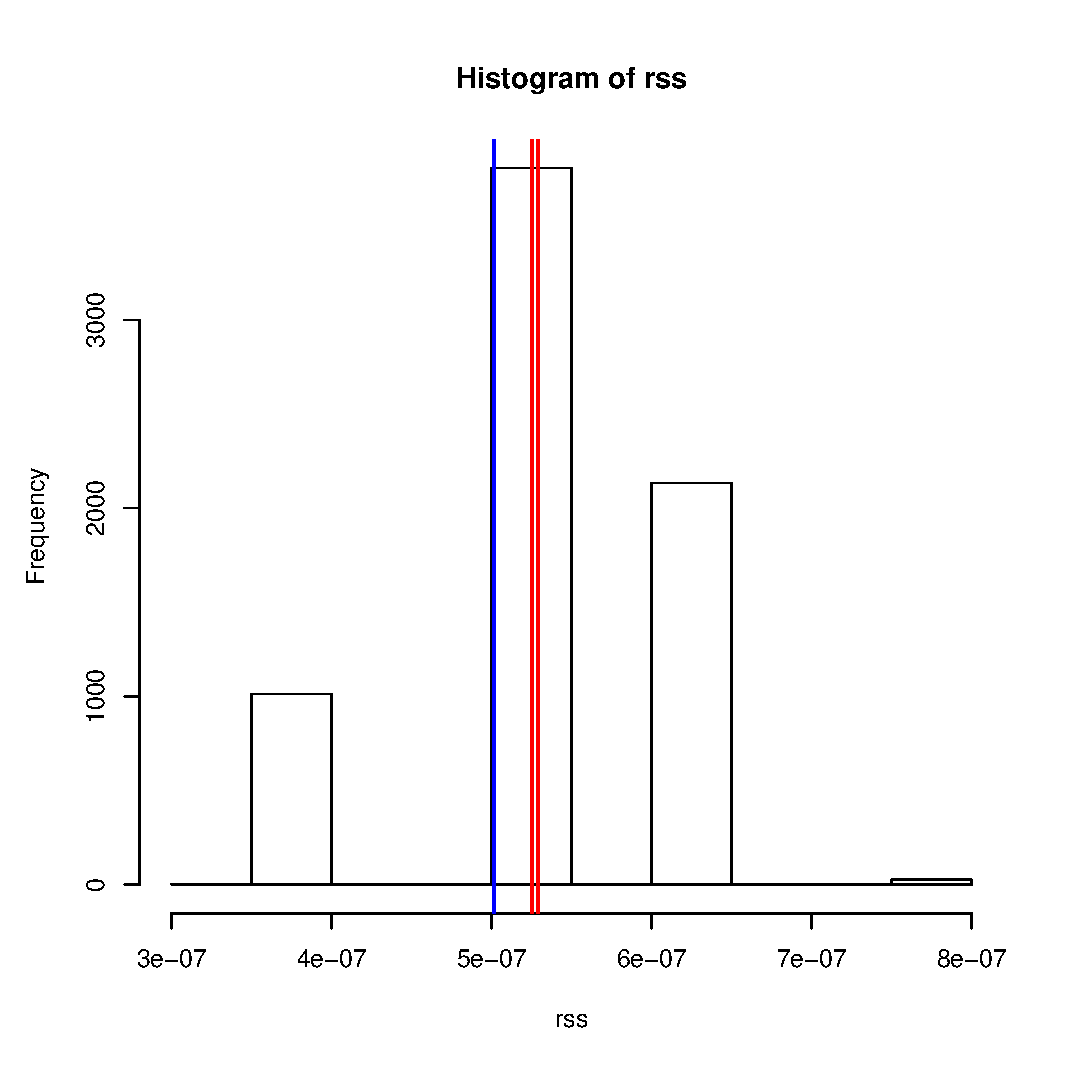
\includegraphics[scale=0.2]{link-5-channel-36.eps}
  \caption{Dataset}
  \label{fig:Dataset}
\end{figure}
\begin{figure}[!ht]
  \centering
  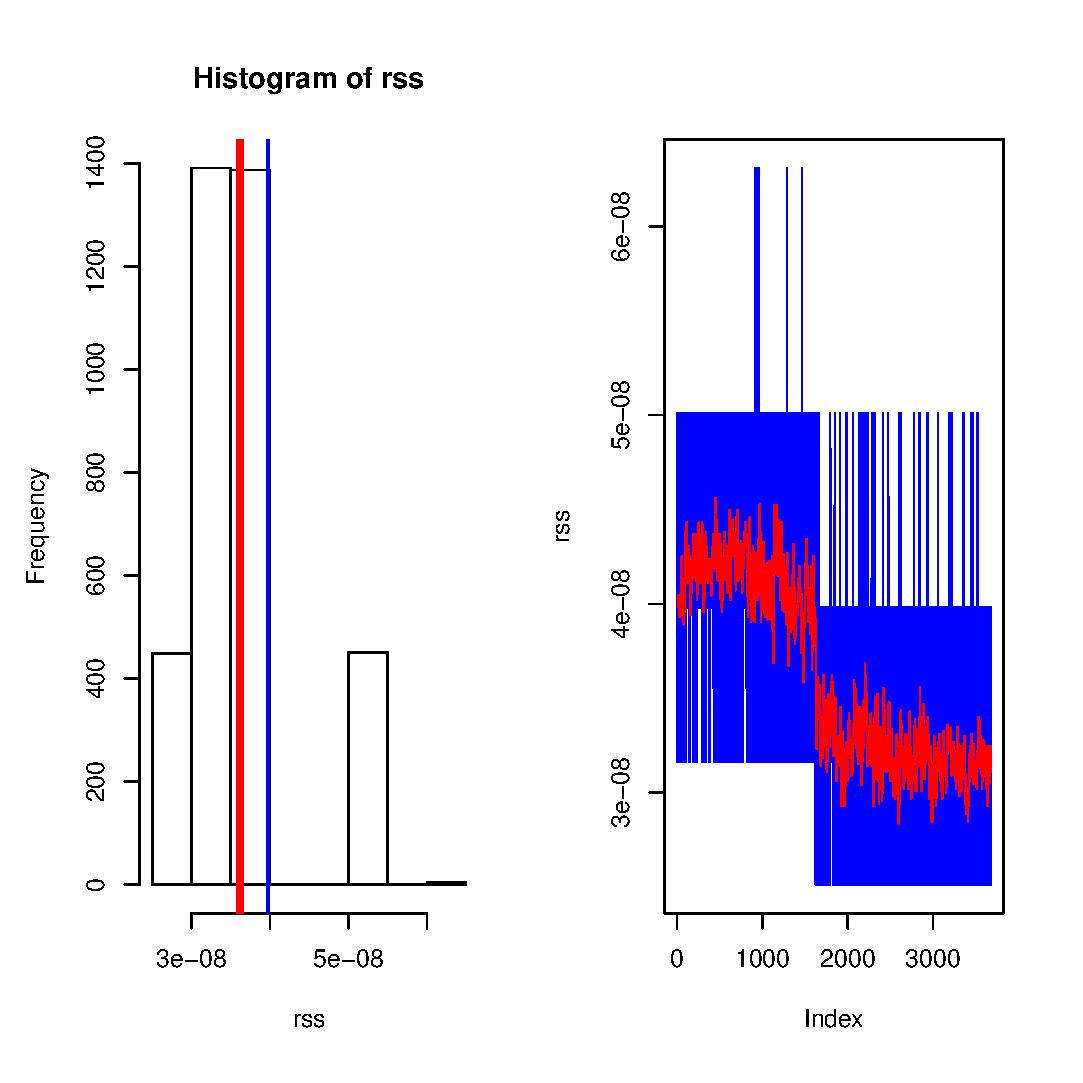
\includegraphics[scale=0.2]{link-5-channel-64.eps}
  \caption{Dataset}
  \label{fig:Dataset}
\end{figure}
\begin{figure}[!ht]
  \centering
  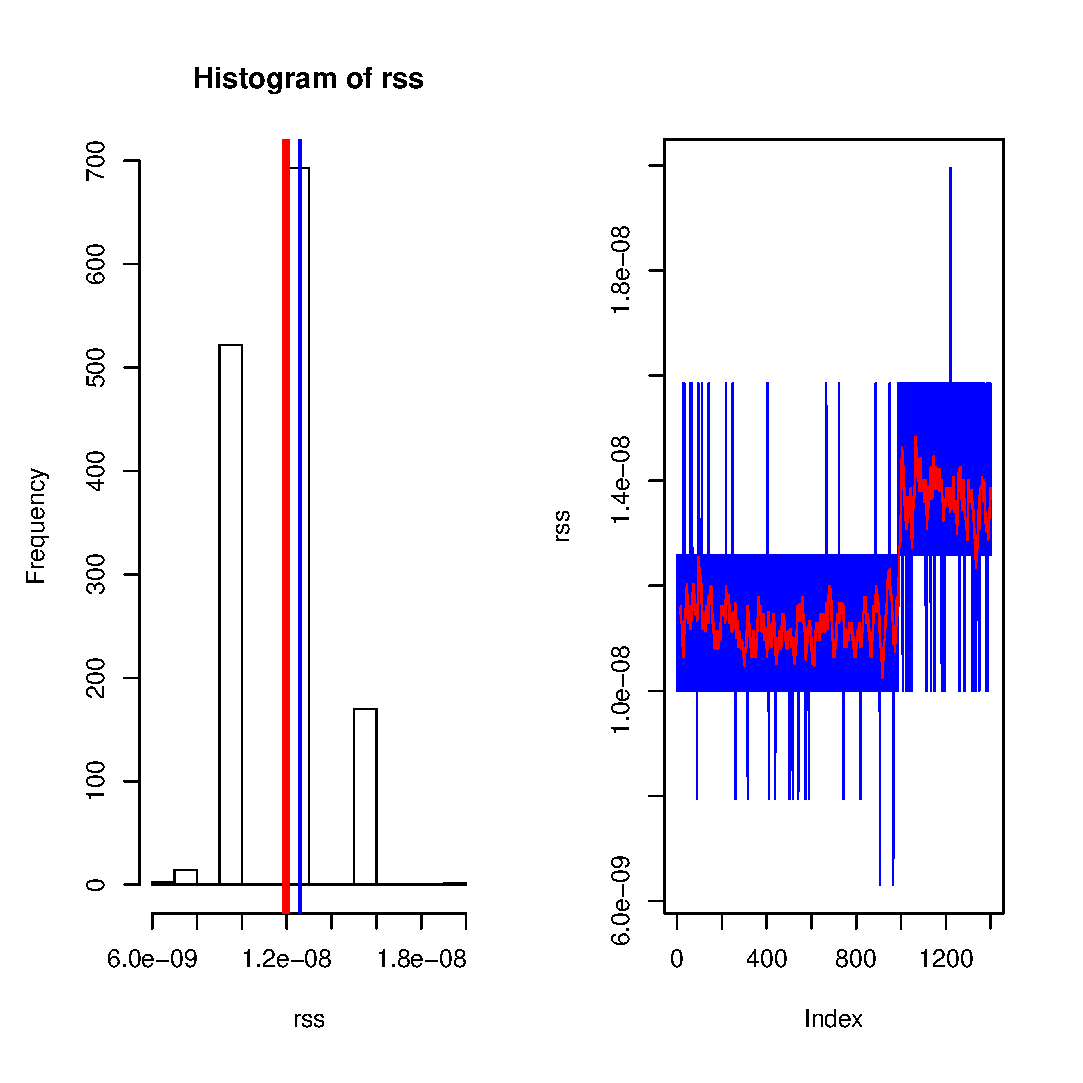
\includegraphics[scale=0.2]{link-5-channel-165.eps}
  \caption{Dataset}
  \label{fig:Dataset}
\end{figure}
\begin{figure}[!ht]
  \centering
  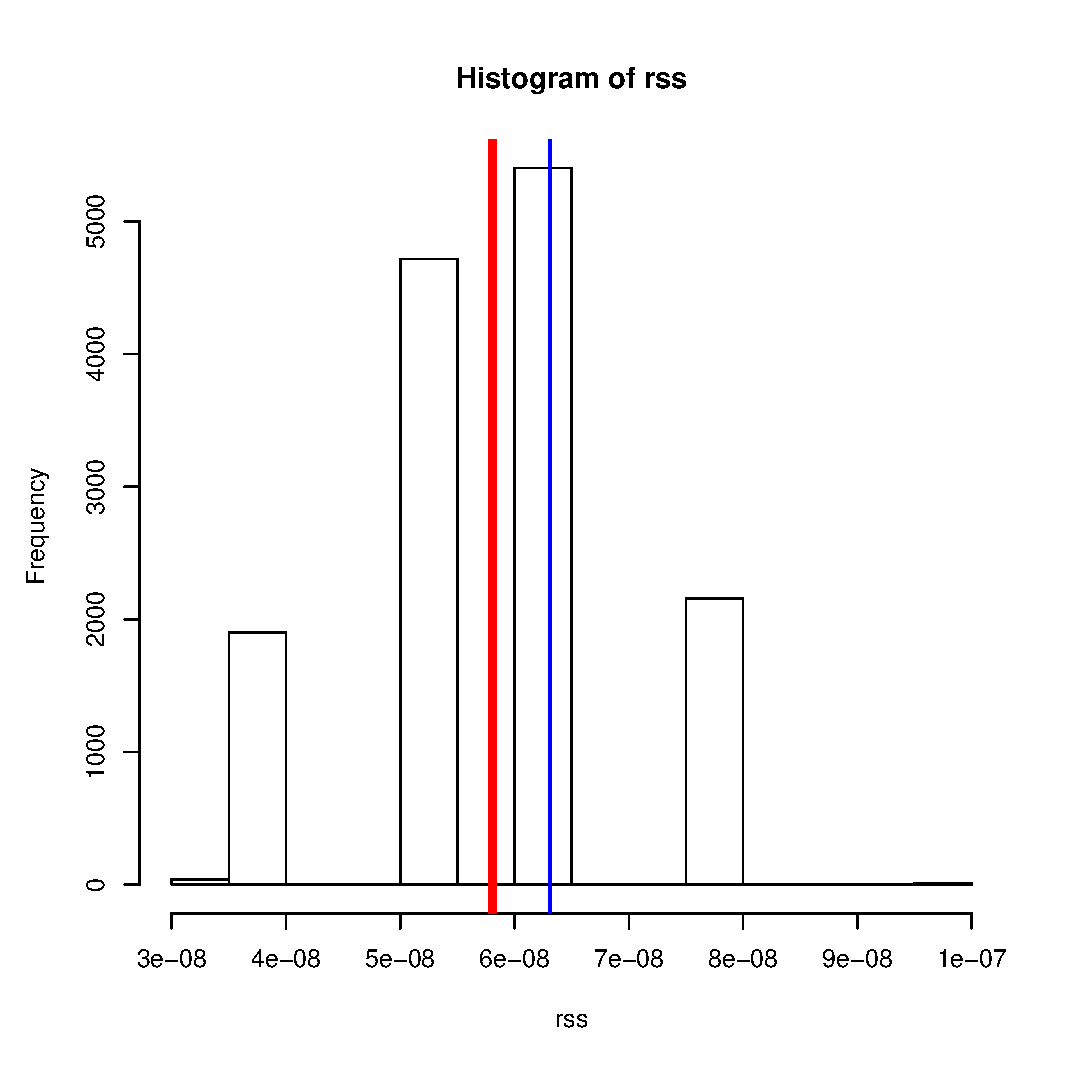
\includegraphics[scale=0.2]{link-14-channel-36.eps}
  \caption{Dataset}
  \label{fig:Dataset}
\end{figure}
\begin{figure}[!ht]
  \centering
  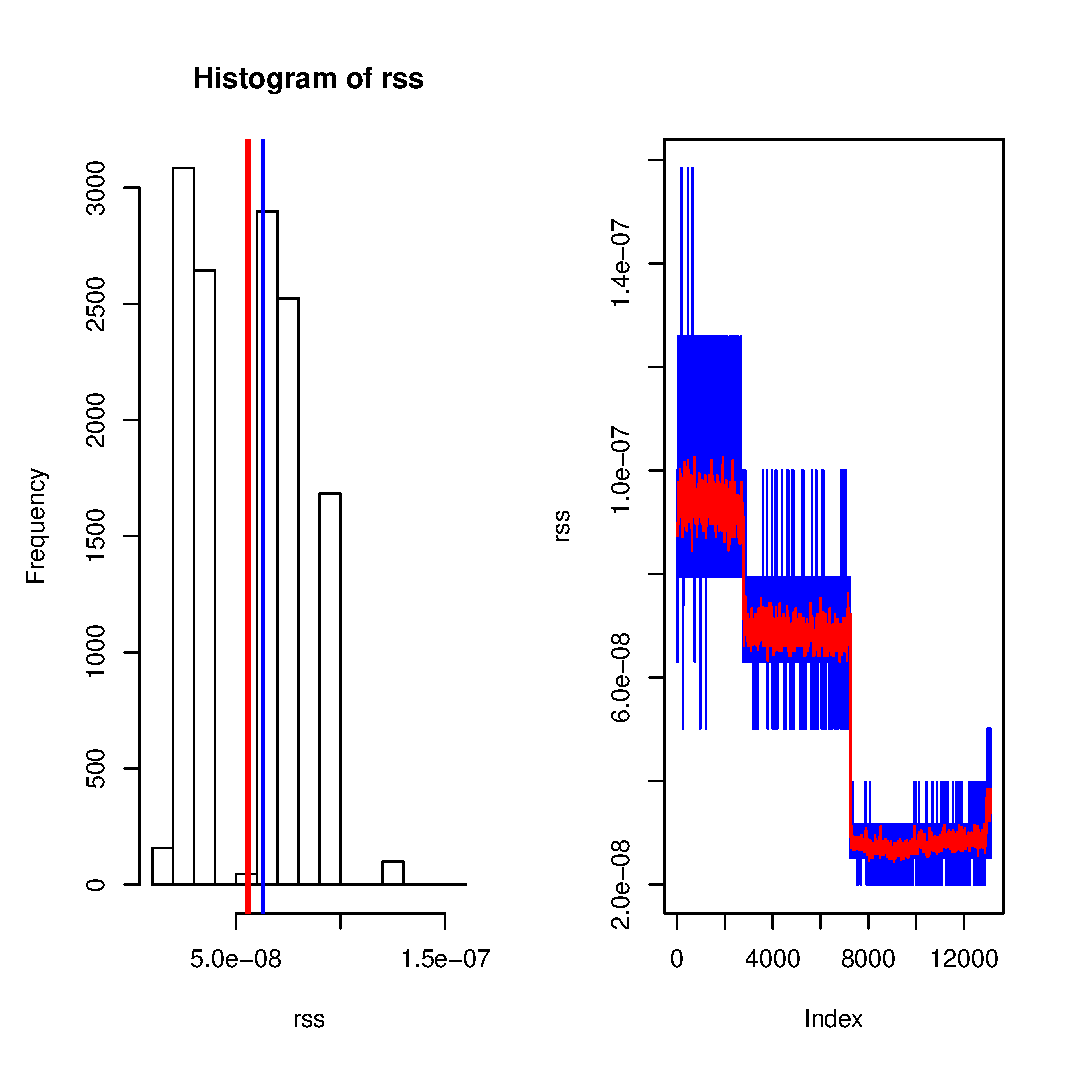
\includegraphics[scale=0.2]{link-14-channel-64.eps}
  \caption{Dataset}
  \label{fig:Dataset}
\end{figure}
\begin{figure}[!ht]
  \centering
  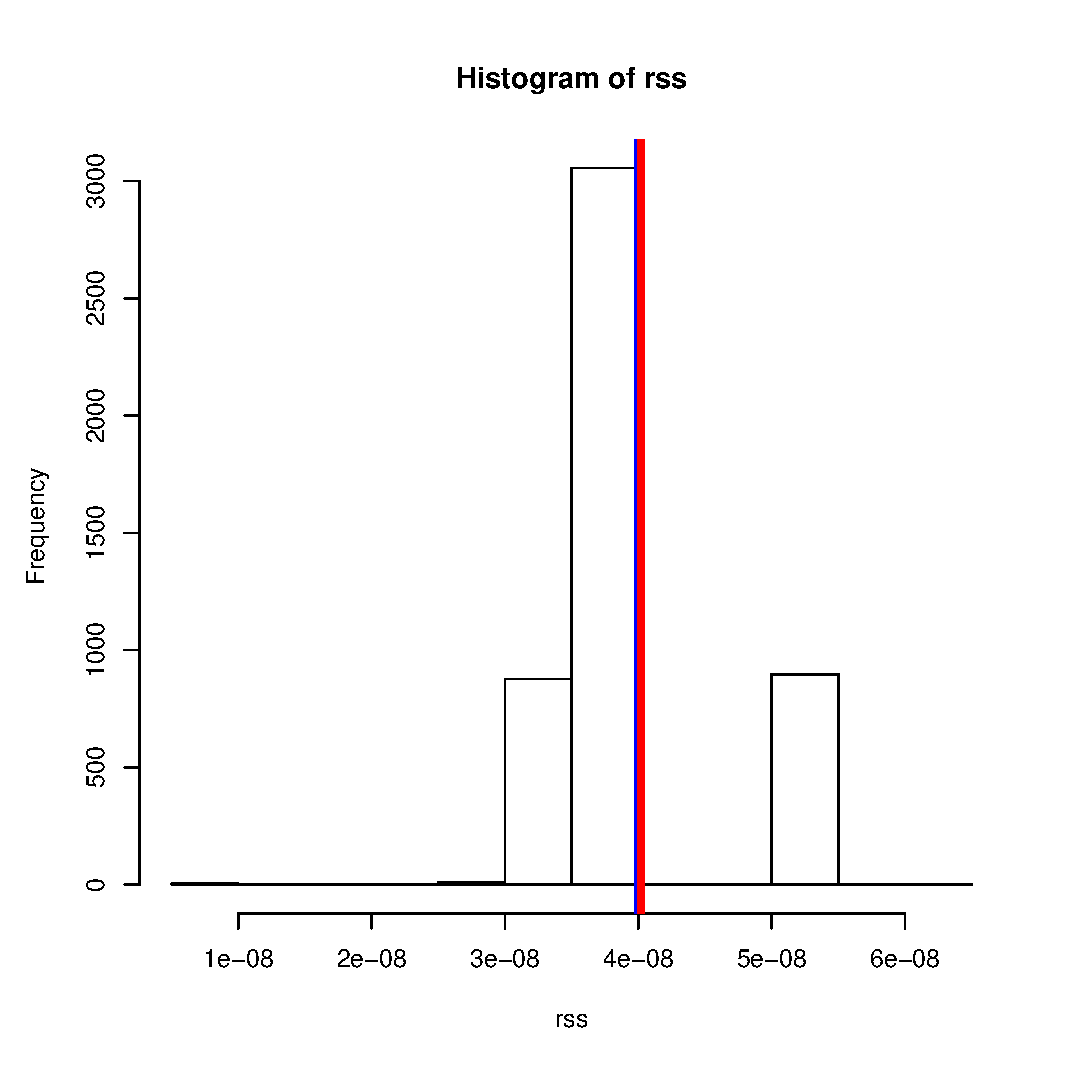
\includegraphics[scale=0.2]{link-14-channel-165.eps}
  \caption{Dataset}
  \label{fig:Dataset}
\end{figure}
\begin{figure}[!ht]
  \centering
  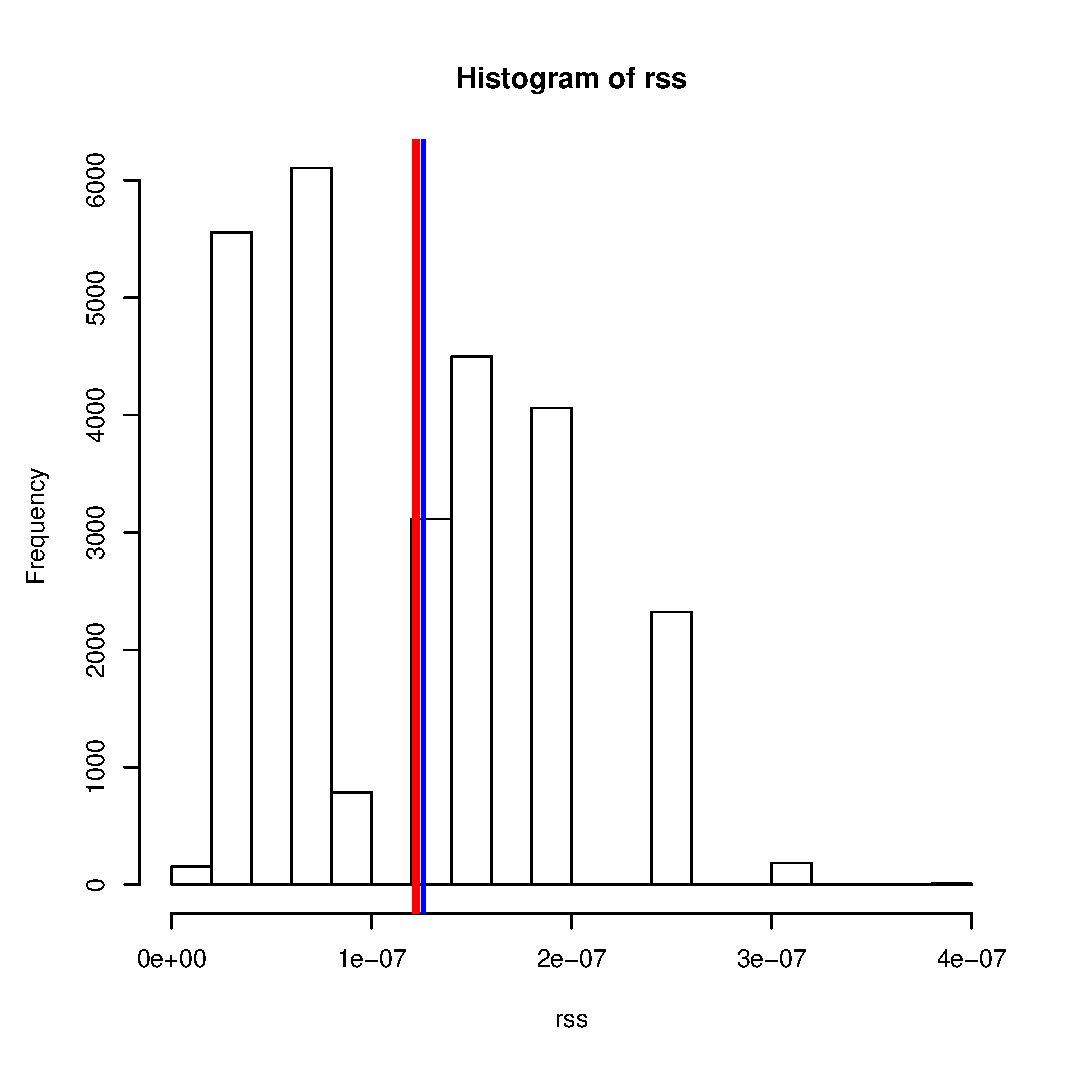
\includegraphics[scale=0.2]{link-35-channel-36.eps}
  \caption{Dataset}
  \label{fig:Dataset}
\end{figure}
\begin{figure}[!ht]
  \centering
  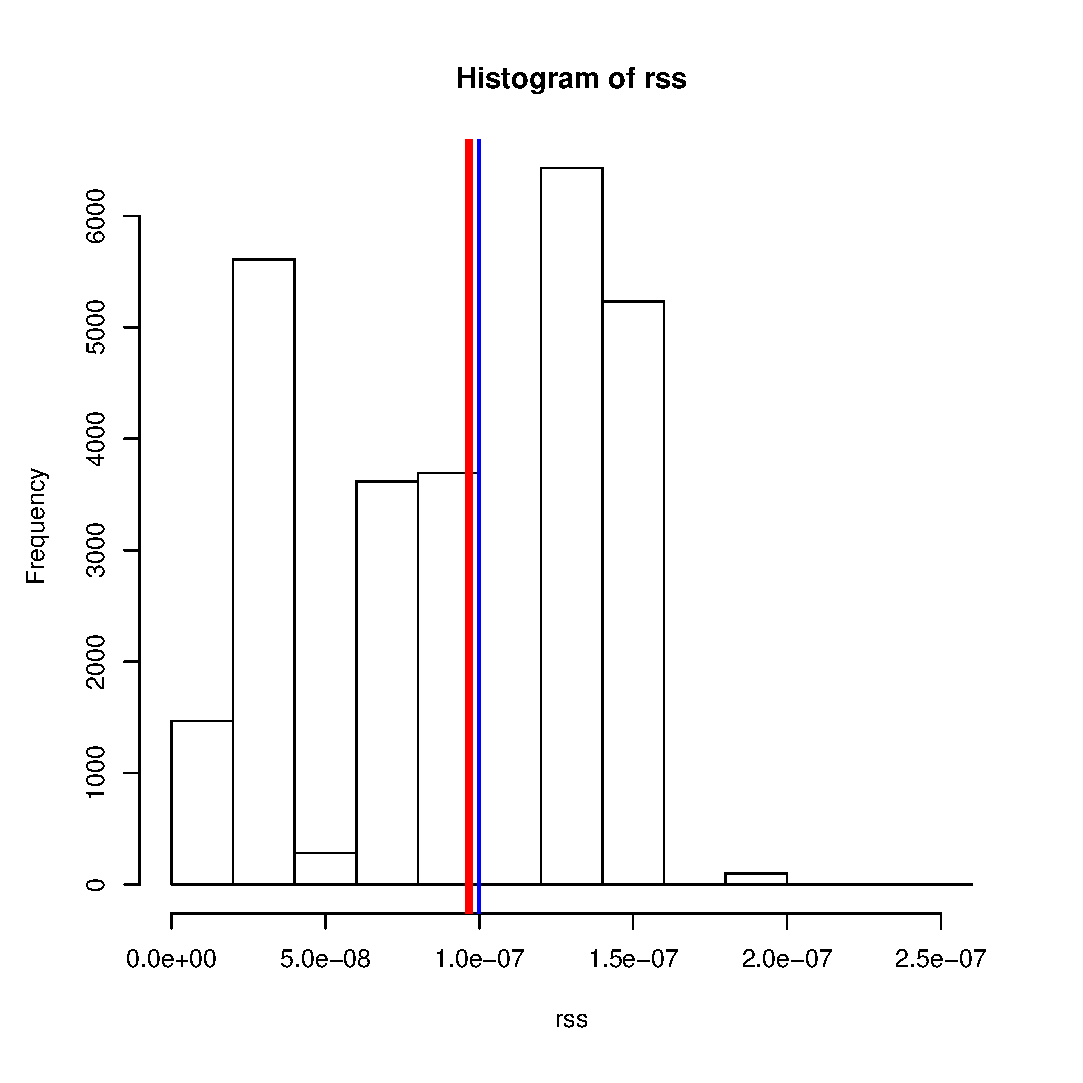
\includegraphics[scale=0.2]{link-35-channel-64.eps}
  \caption{Dataset}
  \label{fig:Dataset}
\end{figure}
\begin{figure}[!ht]
  \centering
  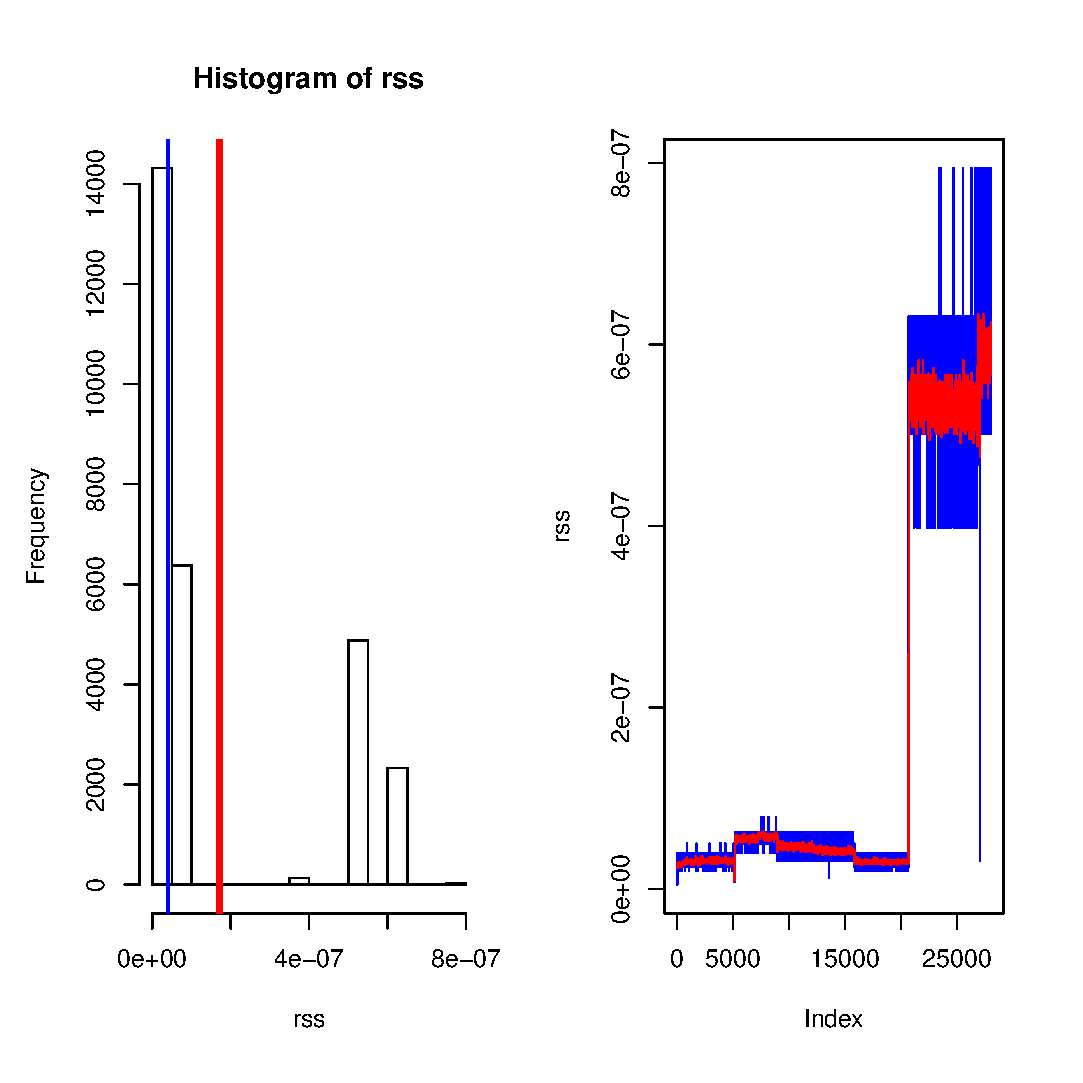
\includegraphics[scale=0.2]{link-35-channel-165.eps}
  \caption{Dataset}
  \label{fig:Dataset}
\end{figure}
\begin{figure}[!ht]
  \centering
  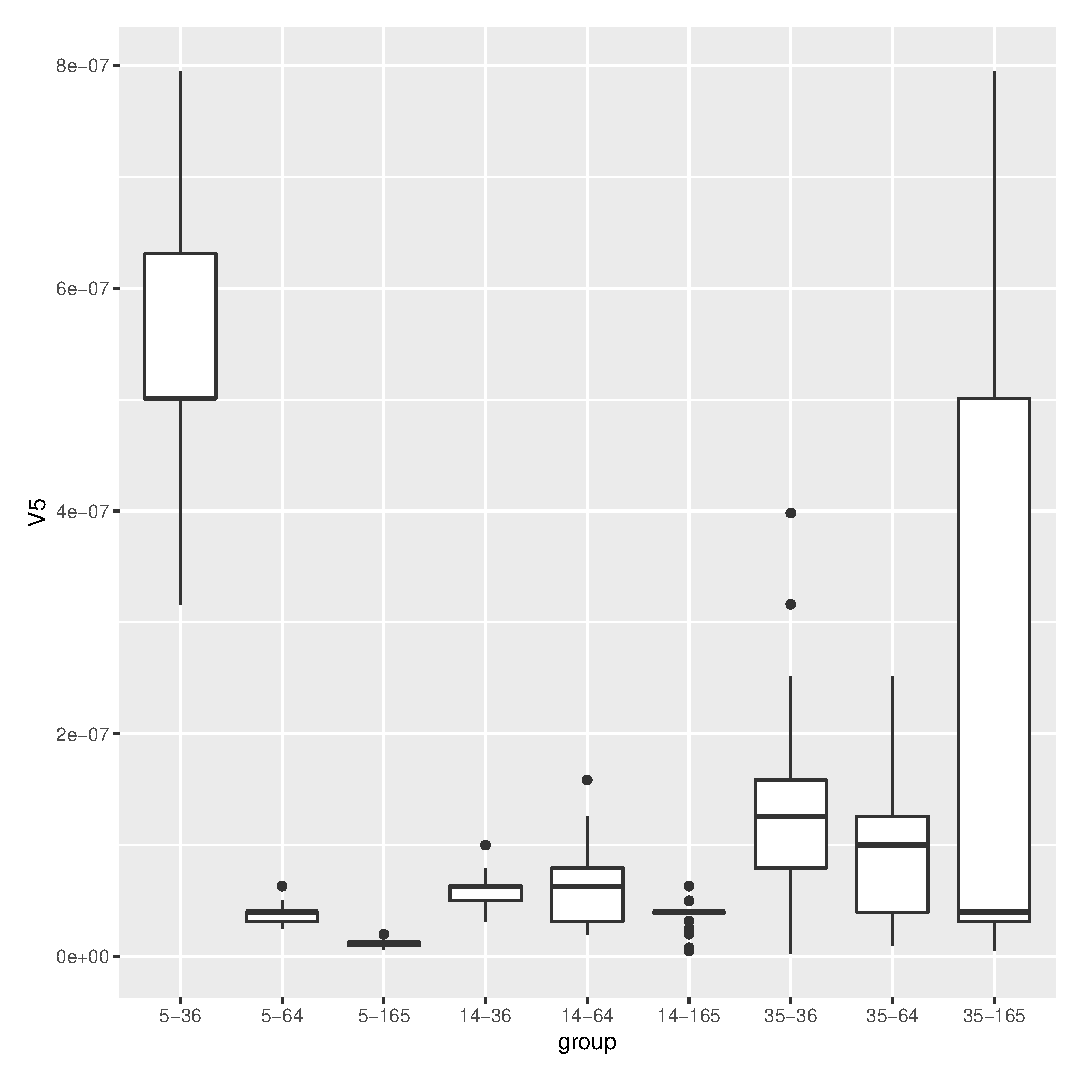
\includegraphics[scale=0.8]{boxplot.eps}
  \caption{Dataset}
  \label{fig:Dataset}
\end{figure}
\subsection{For each combination of link and channel (yes, that means
 1014 combinations, 78 links and 13
channels), compute the MAC frame delivery ratio and the median RSS.}
\begin{figure}[!ht]
  \centering
  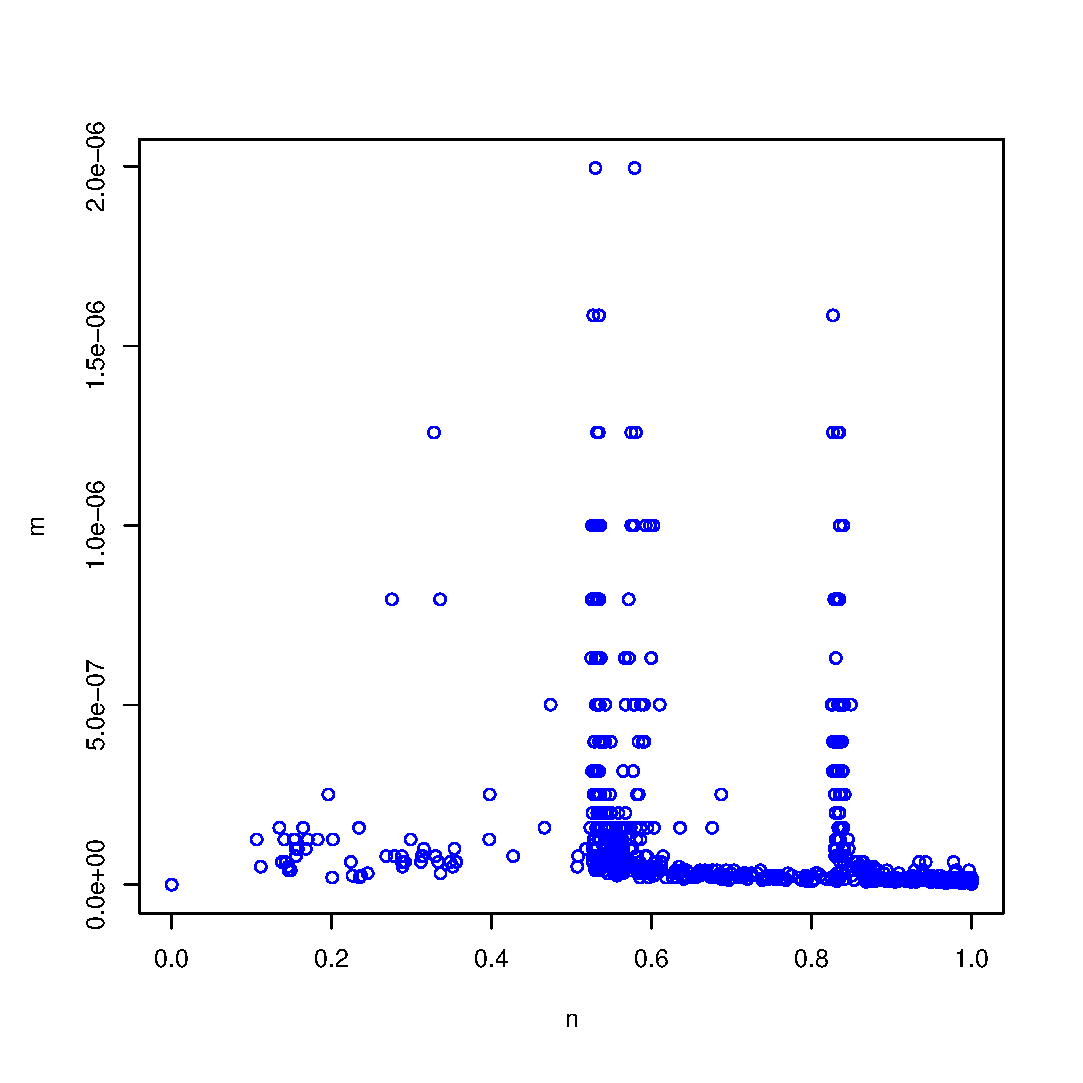
\includegraphics[scale=0.8]{rssvsn.eps}
  \caption{Dataset}
  \label{fig:rssvsn}
\end{figure}
\subsection{Plot}
\par channel versus all corresponding delivery ratios, i.e., you have the channel number on
x-axis and delivery ratios on the y-axis.
\begin{figure}[!ht]
  \centering
  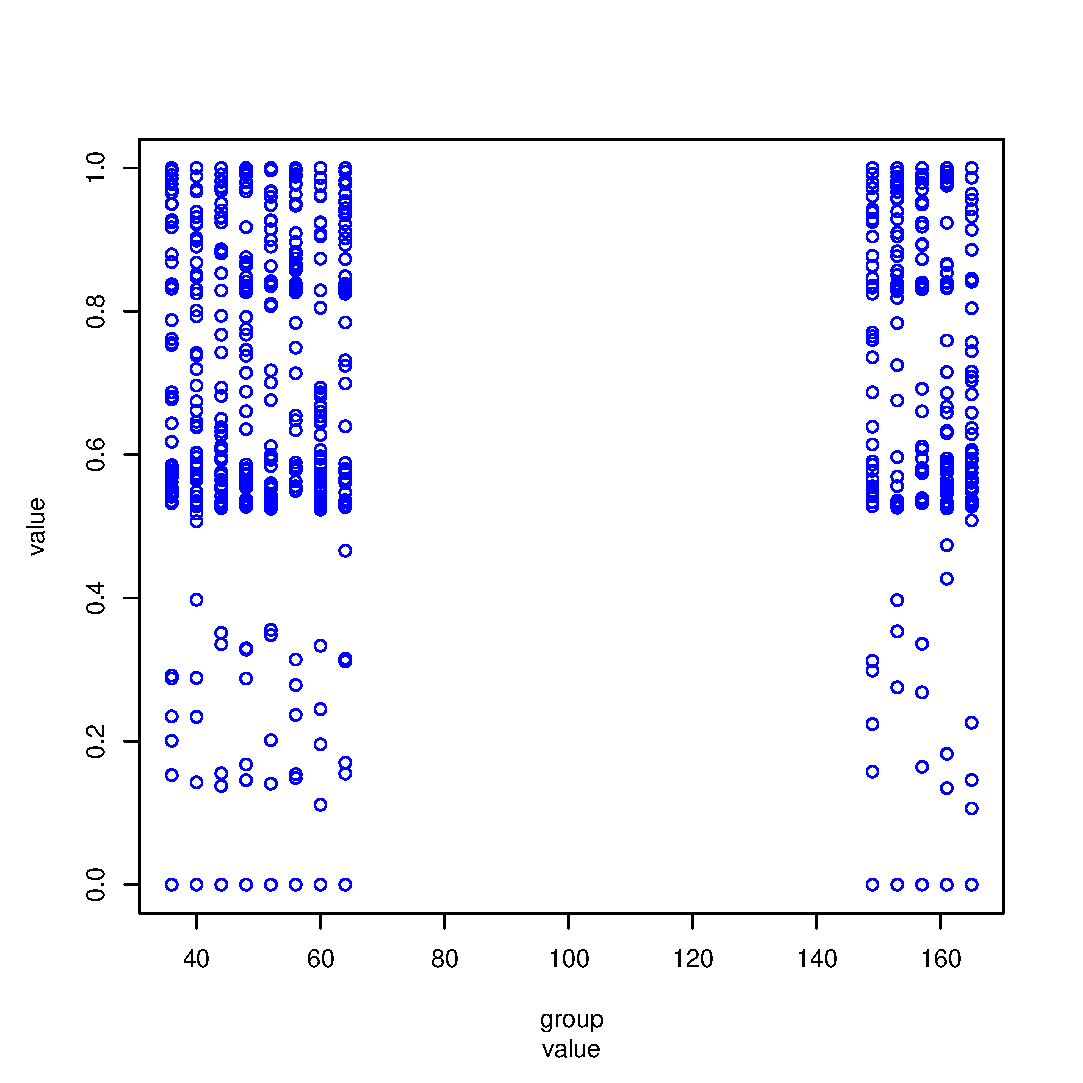
\includegraphics[scale=0.8]{fdrvsch.eps}
  \caption{FDR vs Chanel}
  \label{fig:fdrvsch}
\end{figure}
\par fdr vs link
\begin{figure}[!ht]
  \centering
  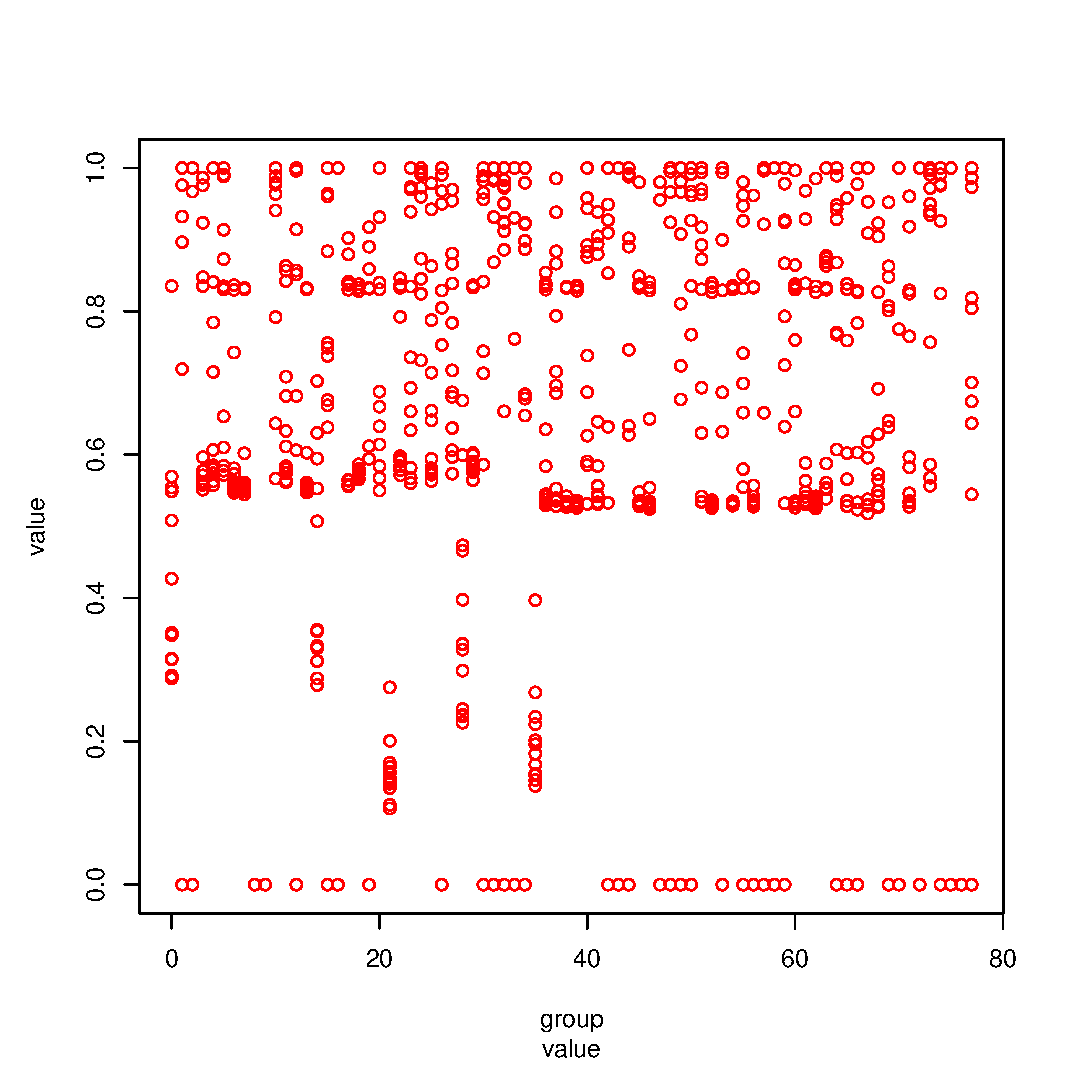
\includegraphics[scale=0.8]{fdrvslink.eps}
  \caption{FDR vs Links}
  \label{fig:fdrvslink}
\end{figure}

\par Chanel vs RSS
\begin{figure}[!ht]
  \centering
  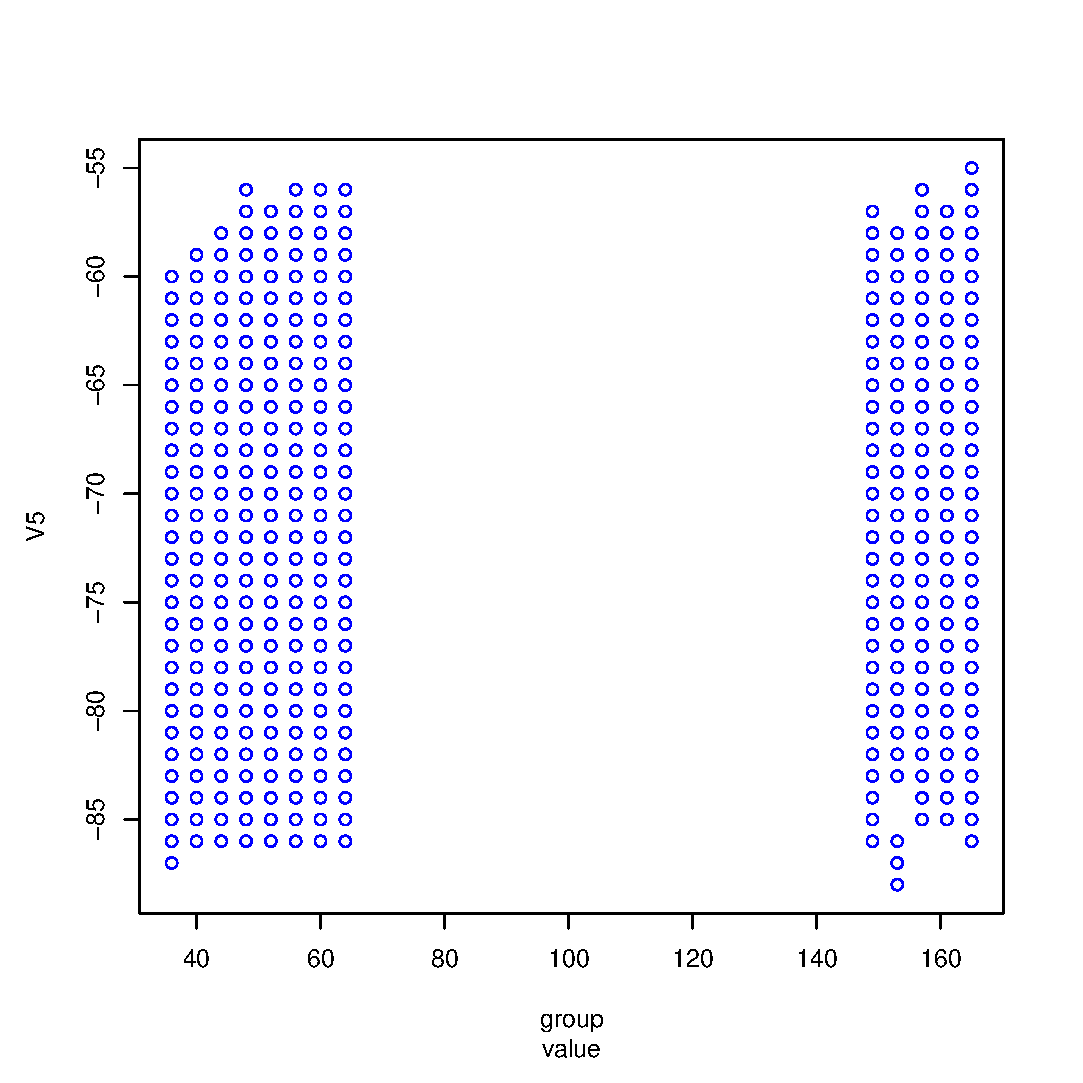
\includegraphics[scale=0.8]{light-rssvsch.eps}
  \caption{RSS vs Chanel}
  \label{fig:rssvsch}
\end{figure}

\par Link vs RSS
\begin{figure}[!ht]
  \centering
  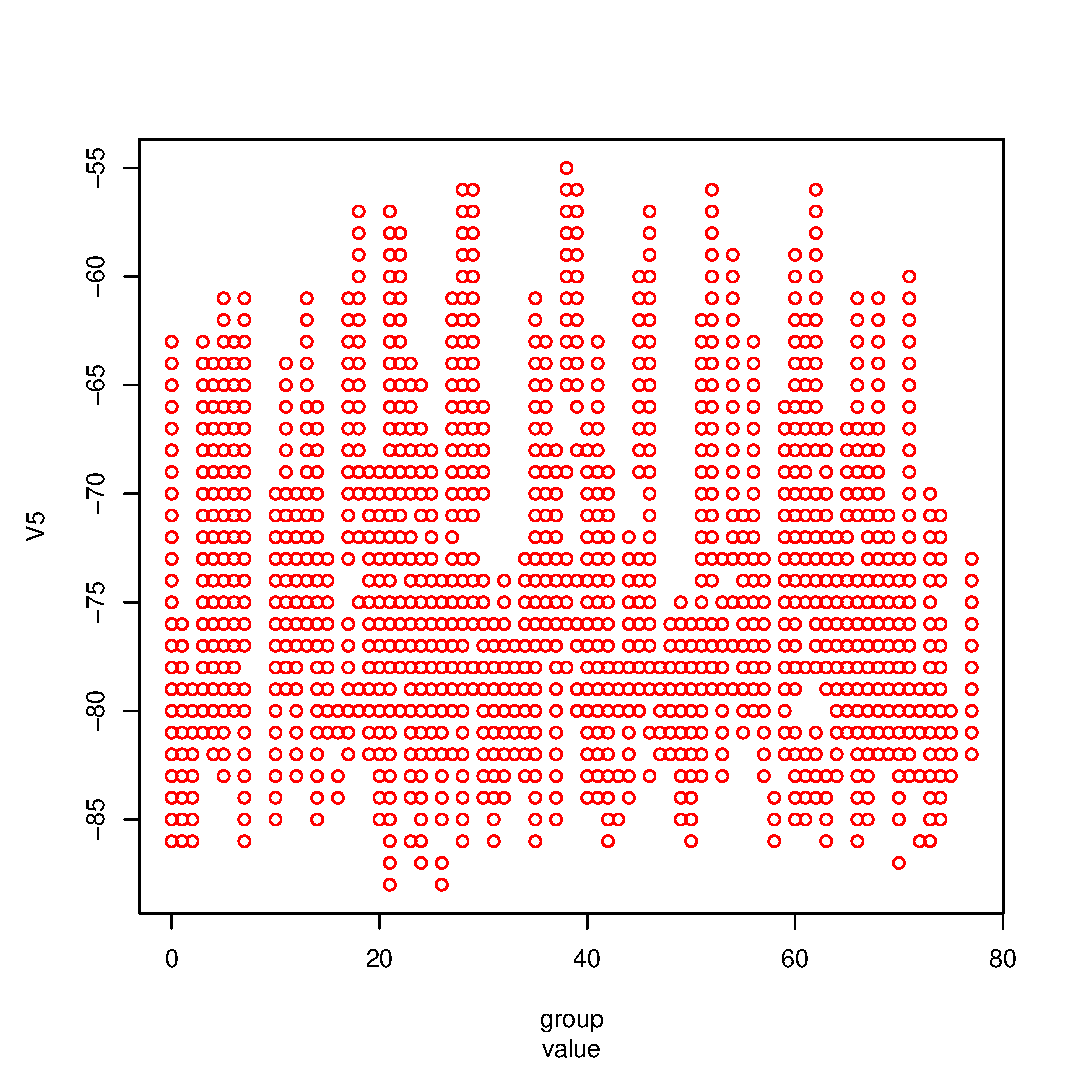
\includegraphics[scale=0.8]{lighter-rssvslink.eps}
  \caption{RSS vs Link}
  \label{fig:rssvslink}
\end{figure}
\subsection{Consider the data for the links 1 and 17. Plot 
the ECDFs for all the RSS values of both links
(i.e., two lines into a single plot). What do you observe?}

%Prints the bibliography
\printbibliography
\end{document}
